%%%% kr-instructions.tex -- version 1.3 (11-Jan-2021)

\typeout{KR2026 Instructions for Authors}

% These are the instructions for authors for KR-26.

\documentclass{article}
\pdfpagewidth=8.5in
\pdfpageheight=11in

\usepackage{kr}

% Use the postscript times font!
\usepackage{times}
\usepackage{soul}
\usepackage{url}
\usepackage[hidelinks]{hyperref}
\usepackage[utf8]{inputenc}
\usepackage[small]{caption}
\usepackage{graphicx}
\usepackage{amsmath}
\usepackage{amsthm}
\usepackage{booktabs}
\usepackage{algorithm}
\usepackage{algorithmic}
\usepackage{ifthen}
\usepackage{xcolor}
\usepackage{graphicx}
\usepackage{tikz-cd}
\usepackage{tikz}
\usetikzlibrary{arrows.meta,positioning,calc,shapes.misc}

\newcommand\algorithmicprocedure{\textbf{procedure}}
\newcommand{\algorithmicendprocedure}{\algorithmicend\ \algorithmicprocedure}
\makeatletter
\newcommand\PROCEDURE[3][default]{%
  \ALC@it
  \algorithmicprocedure\ \textsc{#2}(#3)%
  \ALC@com{#1}%
  \begin{ALC@prc}%
}
\newcommand\ENDPROCEDURE{%
  \end{ALC@prc}%
  \ifthenelse{\boolean{ALC@noend}}{}{%
    \ALC@it\algorithmicendprocedure
  }%
}
\newcommand\CALL[2]{\textsc{#1}(#2)}
\newenvironment{ALC@prc}{\begin{ALC@g}}{\end{ALC@g}}
\makeatother

\urlstyle{same}

% the following package is optional:
%\usepackage{latexsym}

% See https://www.overleaf.com/learn/latex/theorems_and_proofs
% for a nice explanation of how to define new theorems, but keep
% in mind that the amsthm package is already included in this
% template and that you must *not* alter the styling.
\newtheorem{example}{Example}
\newtheorem{theorem}{Theorem}

% Following comment is from ijcai97-submit.tex:
% The preparation of these files was supported by Schlumberger Palo Alto
% Research, AT\&T Bell Laboratories, and Morgan Kaufmann Publishers.
% Shirley Jowell, of Morgan Kaufmann Publishers, and Peter F.
% Patel-Schneider, of AT\&T Bell Laboratories collaborated on their
% preparation.

% These instructions can be modified and used in other conferences as long
% as credit to the authors and supporting agencies is retained, this notice
% is not changed, and further modification or reuse is not restricted.
% Neither Shirley Jowell nor Peter F. Patel-Schneider can be listed as
% contacts for providing assistance without their prior permission.

% To use for other conferences, change references to files and the
% conference appropriate and use other authors, contacts, publishers, and
% organizations.
% Also change the deadline and address for returning papers and the length and
% page charge instructions.
% Put where the files are available in the appropriate places.
%PDF Info Is REQUIRED.
\pdfinfo{
/TemplateVersion (KR.2026.0)
}

\title{Current Limitations of LLM Guided Program Synthesis}
% Comment commands used by Evan. Contain boolean flags to either enable/disable all coments, or enable/disable TODOs and jedi statements.
\newboolean{showcomments}
\setboolean{showcomments}{true}
\newboolean{showjedi}
\setboolean{showjedi}{true}
\newboolean{showtodos}
\setboolean{showtodos}{false}
\newcommand{\editcomment}[2][red]{\ifthenelse{\boolean{showcomments}}{{\color{#1}$\bigl[$\bgroup\em #2\egroup$\bigr]$}}{}}
\newcommand{\note}[1]{\editcomment[blue]{#1}}
\newcommand{\todo}[1]{\ifthenelse{\boolean{showtodos}}{\editcomment{{\bf TODO:} #1}}}
% Evan likes to review "jedi" statements, that should capture the essence of a paragraph (i.e. how would Yoda convey the point of a paragraph?). Should be able to just read the jedi statements to get all the important points of a paper.
\newcommand{\jedi}[1]{\ifthenelse{\boolean{showjedi}}{\editcomment[cyan]{#1}}{}}

\newcommand{\ie}{\textit{i.e.}~}
\newcommand{\eg}{\textit{e.g.}~}

% Note(klinvill): \xspace tries adds a space after uses of `\lang` when
% reasonable. The package's creator recommends not using xspace
% (https://tex.stackexchange.com/questions/86565/drawbacks-of-xspace/86620#86620),
% but I believe that the LaTeX behavior of eating spaces will be more surprising
% to co-authors than the occassional weird spacing introduced by xspace.
% Language Name
%---------------
\newcommand{\lang}{TSQL\xspace}

\newcommand{\bigstep}{\Downarrow}
% Formatting
%---------
\newcommand{\kw}[1]{\texttt{#1}} %keywords
\newcommand{\code}[1]{{\tt #1}}
\newcommand{\C}[1]{\code{#1}}
\newcommand{\tuplee}[1]{\langle #1 \rangle}
\newcommand*{\rom}[1]{\expandafter\romannumeral #1}
\newcommand{\spc}[0]{\quad}
\newcommand{\ALT}{~\mid~}
\newcommand{\ALTE}{\spc\mid\spc}
\newcommand{\conj}{~\wedge~}
\newcommand{\disj}{~\vee~}
\newcommand{\Iv}{I_{\mathrm{le}}^v}
\newcommand{\cle}{\mvc_{\mathrm{le}}}
\newcommand{\blue}[1]{\textcolor{Blue}{#1}}
\newcommand{\brown}[1]{\textcolor{Brown}{#1}}


% Math env
%-----------
\newenvironment{nop}{}{}
\newenvironment{smathpar}{
\begin{nop}\small\begin{mathpar}}{
\end{mathpar}\end{nop}\ignorespacesafterend}

% Relational algebra notation for use in denotational semantics
%--------------
\newcommand{\denote}[1]{\llbracket #1 \rrbracket}
\newcommand{\semof}{\denote}
\newcommand{\projectOp}{\pi}
\newcommand{\project}[2]{\projectOp_{#1}(#2)}
\newcommand{\filterOp}{\sigma}
\newcommand{\filter}[2]{\filterOp_{#1}(#2)}
\newcommand{\joinOp}{\bowtie}
\newcommand{\join}[3]{#1 \bowtie_{#3} #2}
\newcommand{\aggfun}{\mathcal{G}}
\newcommand{\agg}[2]{|#2|_{#1}}
\newcommand{\orderOp}{\omega}
\newcommand{\orderby}[2]{\orderOp_{#1}(#2)}
\newcommand{\groupby}[2]{|#2|_{#1}}
\newcommand{\renameOp}{\rho}
\newcommand{\rename}[2]{\renameOp_{#1}(#2)}
\newcommand{\bind}{\gg=}


\newcommand{\concatRows}{\mathbin{++}}
\newcommand{\concatCols}{\oplus}

\newcommand{\db}{\mathcal{D}}
\newcommand{\denotedb}[1]{\denote{#1}_{\db}}

% Inference rule notation
\newcommand{\RULE}[3]{\inferrule*[Right=#1]{#2}{#3}}
\newcommand{\rulelabel}[1]{\textrm{\sc {#1}}}

\newcommand{\hole}{\square}
\newcommand{\collection}[1]{\overline{#1}}

\newcommand{\cstr}{\mathcal{C}}
\newcommand{\cols}{\sf cols}
\newcommand{\fresh}{\sf fresh}

% Custom commands
\newcommand{\lm}{\mathcal{L}}
\theoremstyle{definition}
\newtheorem{exmp}{Example}[section]
\newtheorem{thrm}{Theorem}[section]
\newtheorem{lma}{Lemma}[section]


% Single author syntax
\iffalse % (remove the multiple-author syntax below and \iffalse ... \fi here)
\author{%
    Author name
    \affiliations
    Affiliation
    \emails
    email@example.com    % email
}
\fi
% Multiple author syntax
% \author{%
% First Author$^1$\and
% Second Author$^2$\and
% Third Author$^{2,3}$\and
% Fourth Author$^4$ \\
% \affiliations
% $^1$First Affiliation\\
% $^2$Second Affiliation\\
% $^3$Third Affiliation\\
% $^4$Fourth Affiliation \\
% \emails
% \{first, second\}@example.com,
% third@other.example.com,
% fourth@example.com
% }

\author{Anonymous Author(s)}

\begin{document}

\maketitle

\begin{abstract}

Large Language Models (LLMs) exhibit strong performance for program synthesis tasks including text-to-SQL, up to 86.6\% accuracy on the Spider 1.0 benchmark. The top-performing methods bridge the semantic gap between natural language and SQL by using prompt engineering, fine-tuning, or in-context learning techniques; however, these purely neural techniques remain prone to hallucinations.
Existing symbolic approaches to improve accuracy on program synthesis tasks generally rely on post-hoc verification, which fails to constrain unproductive path exploration, or constrained decoding techniques that rely on the underlying distribution of the model.
The effectiveness of symbolic guidance under complex queries and the semantic ambiguity inherent in text-to-SQL benchmarks, however, remains unclear.
In this work, we study the \emph{``ground truth''} errors made by LLMs in the text-to-SQL task looking at both fine-tuned models and a general-purpose model optimized for code generation.
We study the incremental prediction errors LLMs make and find that errors can be grouped into six error categories, three of which are amenable to simple symbolic fixes.
Importantly, we find that for some error types, correct predictions do not rank near the top of the LLMs likely predictions, implying that \emph{constrained decoding alone is insufficient} to guide synthesis on hard problems.
Our findings provide interpretable insight into where LLMs fail and suggest promising, neuro-symbolic directions for improving LLM guided program synthesis.

% Large Language Models (LLMs) have exhibited strong performance on program synthesis tasks such as text-to-SQL, achieving up to $\sim$87\% accuracy on state-of-the-art challenges such as the Yale Semantic Parsing (Spider). However, most of the top-performing methods bridge the semantic gap between natural language and SQL using clever prompt engineering, fine-tuning, or in-context learning techniques.
% All these methods rely on the LLM to generate the entire SQL query and then perform a post-hoc verification step to check the validity of the generated query. Logically, this approach does not constrain the LLM from generating paths that lead to ``semantic deadends''. Further, constrained decoding helps alleviate this issue by checking if it can find a valid continuation within the program space of the next predicted token. However, the effectiveness of this approach under complex queries and semantic ambiguity such as in SQL is questionable. To this end, we observe that the so called \emph{``ground truth'' mistakes that LLMs make using both a fine-tuned and prompt-engineered model with constrained decoding prove insufficient} to address \wip{<z>} of these categories.
% Our findings provide interpretable insight into where LLMs fail and suggest promising, neuro-symbolic directions for improving LLM guided program synthesis.

\end{abstract}

% \begin{figure*}
%     \centering
%     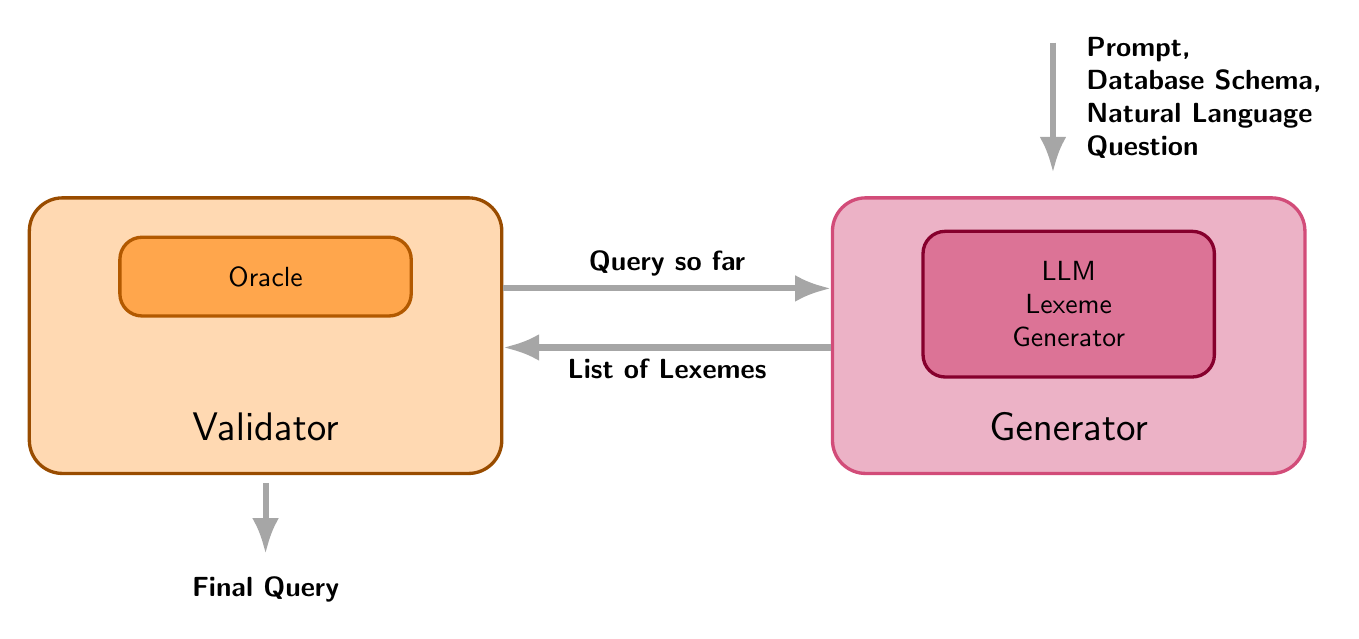
\begin{tikzpicture}[
  font=\sffamily,
  box/.style={rounded corners=12pt, very thick, inner sep=10pt},
  innerbox/.style={rounded corners=8pt, very thick, inner sep=8pt},
  arrow/.style={-{Latex}, line width=2.2pt, draw=gray!70},
  arrowrev/.style={{Latex}-, line width=2.2pt, draw=gray!70},
]

% --- Left: Validator ---
\node[box, draw=orange!60!black, fill=orange!30, minimum width=6cm, minimum height=3.5cm] (validator) at (0,0) {};
\node[innerbox, draw=orange!70!black, fill=orange!70, minimum width=3.7cm, minimum height=1cm] (oracle) at ($(validator.center)+(0,0.75)$) {Oracle};
\node[font=\sffamily\Large] at ($(validator.center)+(0,-1.15)$) {Validator};

% --- Right: Generator ---
\node[box, draw=purple!70, fill=purple!30, minimum width=6cm, minimum height=3.5cm] (generator) at (10.2,0) {};
\node[innerbox, draw=purple!70!black, fill=purple!55, minimum width=3.7cm, minimum height=1.85cm, align=center] (llm) at ($(generator.center)+(0,0.40)$) {LLM\\Lexeme\\Generator};
\node[font=\sffamily\Large] at ($(generator.center)+(0,-1.15)$) {Generator};

% --- Between arrows ---
\draw[arrow] ($(validator.east)+(0,0.60)$) -- node[above, font=\sffamily\bfseries] {Query so far} ($(generator.west)+(0,0.60)$);
\draw[arrowrev] ($(validator.east)+(0,-0.15)$) -- node[below, font=\sffamily\bfseries] {List of Lexemes} ($(generator.west)+(0,-0.15)$);

% --- Top input arrow into Generator ---
\draw[arrow] ($(generator.north)+(-0.2,1.95)$) -- ($(generator.north)+(-0.2,0.30)$);
\node[anchor=west, align=left, font=\sffamily\bfseries] at ($(generator.north)+(0.1,1.25)$)
{Prompt,\\Database Schema,\\Natural Language\\Question};

% --- Bottom output arrow from Validator ---
\draw[arrow] ($(validator.south)+(0,-0.10)$) -- ($(validator.south)+(0,-1)$);
\node[font=\sffamily\bfseries] at ($(validator.south)+(0,-1.45)$) {Final Query};

\end{tikzpicture}
%     \caption{The overall system architecture. The Language Model Generator is prompted to generate a SQL query given a database schema and natural language question. The generator returns a list of lexemes to the Validator which incrementally validates the most probable lexeme against the gold one and corrects the generator if there is a mismatch.}
%     \label{fig:overview}
% \end{figure*}

\section{Introduction}
\jedi{Symbolic techniques could be used to address LLM's weakness for program synthesis tasks: LLMs make good guesses on average, but lack correctness guarantees.}
The advent of Large Language Models (LLMs) are increasingly used as program generators to synthesize working code. In contrast to other program synthesis techniques, LLMs are scalable to larger and more complex programs; however, they struggle with self-correction and can get stuck down an incorrect path that, ultimately, will not yield correct code. Conventional program synthesis techniques use symbolic reasoning to produce correct code but are limited in scalability. 


LLMs are used to write code and synthesize programs - they can be quite good at it but they suffer from hallucinations ... contrast this with other program synthesis techniques

Let's observe the mistakes LLMs do make

We categorize them and see oh wow we can use some symbolic techniques that improve LLM generation 


We hypothesize that an integration of insights and techniques from conventional symbolic reasoning techniques can be applied at inference time to guide LLMs to more promising search spaces. 

To evaluate the validity of our hypothesis, we focus our efforts on tackling a subspace of the program synthesis domain, the text-to-SQL task, as it is easier to verify and validate a query's correctness. The text-to-SQL task is concerned with generating valid SQL queries that correctly answers a natural language question for a given schema or workflow. For example, for the question "How many clubs are there?" for a given schema the corresponding gold SQL query is "SELECT count(*) FROM club" \cite{spider-sql}. We hypothesize that the insights gained from this work will be further applicable in broader code generation tasks. 

Our contributions are as follows:
\begin{itemize}
    \item We present a taxonomy of error categorization for LLM mistakes during decoding. 
    \item We show that two mistake categories are amenable to a handful of symbolic repair techniques.
    \item We show that the combination of constrained decoding and symbolic repair techniques could help fix FIXME mistakes an LLM makes. 
\end{itemize}


% We perform supervised finetuning on an LLM (Qwen-7B?) on the Spider 1.0 dataset using a DSL (TSQL) for easier evaluation and give the LLM a database schema and natural language question and prompt the LLM to generate a valid TSQL query that answers the NL question. Using the SFT model, we generate a candidate query lexeme by lexeme. As the LLM is generating lexemes, we compare each with the gold lexeme. If there is a mismatch, we correct the LLM's behavior by providing the generator with the gold lexeme and continue generating lexemes. We observe that the SFT model produces the correct query FIXME (85) percent of the time; however, the inclusion of symbolic techniques would increase the percentage of correctly generated queries to FIXME (95) percent.

% We observe several errors in the LLM's generation that can be corrected through simple symbolic fixes.  

\section{Related Work}
Prior research has explored SQL synthesis using classic approaches, such as enumerative search, to produce correct queries~\cite{scythe,patsql}.
These works focus on pruning the search space either through additional information provided by the user, such as the constants that are allowed to appear in a query~\cite{scythe,patsql}, or through pruning unproductive paths~\cite{scythe,patsql}.
They often include soundness and bounded completeness guarantees, but struggle to scale to larger, more complex queries.

Other research instead foregoes guarantees for empirical results.
Many recent works focus on leveraging Large Language Models (LLMs) to produce SQL queries~\cite{dail-sql}.
They have performed well empirically, reaching test suite accuracies of up to 86.6\%~\cite{dail-sql} against the Spider SQL dataset~\cite{spider-sql}. FIXME MiniSeek 91.2 but no reference

Some prior works build off the strengths of both approaches, using probabilistic models to guide search while verifying the correctness of produced candidates.
These prior works either require white-box access to probabilistic models~\cite{probabilistic-model-synthesis,ml-pbe}, or treat models as program candidate oracles~\cite{llm-cegis}, or apply a hybrid approach that combines both methods~\cite{llm-enumerative-search}.
However, all these works use probabilistic models to generate full candidate programs before evaluating them.
This leaves a large search space for the probabilistic model to categorize.

In contrast, we observe that LLMs are inherently next token predictors, rather than full sequence predictors.
We leverage this insight to guide LLM search using lexeme level guidance which provides early guidance for the LLM to avoid unproductive search paths.

With regards to ChopChop, A. our insights are complimentary to ChopChop 
B. they observed that once an LLM made a mistake...it was too late to go back and fix it...."The type system implemented in our semantic pruner will prevent
the assignment to divisors, but it will still allow line 2." so LLM commit to its solution so it is useful to mitigate these types of errors before it is too late
C. constrained decoding is known to skew the underlying distribution
D. The pruners in ChopChop seem a bit unrealistic to create but I guess this is theoretical
So ChopChop enforces semantic validity when generating queries...in theory...but this requires you to create pruners...and you still run into the issue of an LLM makes a mistake and you reach a point where its too late to correct it...so other symbolic fixes? I mean you could still use this...ChopChop still wouldn't work because the candidates aren't in top-k...you would need to have the model learn some more patterns/ clause constraints





% \section{TSQL}
% \subsection{TSQL Syntax}

SQL's design has some well-known drawbacks including that the syntax does not reflect data flow~\cite{pipesql}.
This presents a challenge to incremental query validation which we perform in reverse data flow order. To this end, we introduce a novel Domain Specific Language (DSL) based on SQL which we call TSQL to allow for validation of partial prefixes when autoregressively generating queries. The syntax of TSQL is shown in \ref{fig:syntax}.


\begin{figure*}[ht]
\begin{mathpar}
    \begin{array}{lclcl}

      q & \in & \kw{Queries} & \Coloneqq ~~ &
        %
        \kw{PROJECT} ~ [\kw{DISTINCT}] ~ \overline{ac} ~ \kw{FROM} ~ q \spc
        \blue{\project{\kw{distinct}? \overline{ac}}{q}} 
        %
        \ALT \kw{SELECT WHERE} ~ \phi ~ \kw{FROM} ~ q \spc
        \blue{\filter{\phi}{q}}\\
        %
        &&&&\ALT \kw{JOIN} ~ q ~ \kw{WITH} ~ q ~ \kw{ON} ~ {\overline{\phi}} \spc
        \blue{\join{q}{q}{\overline{\phi}}} \spc
        %
        \ALT \kw{ORDER BY} ~ {\overline{oc}} ~ \kw{FROM} ~ q \spc
        \blue{\orderby{{\overline{oc}}}{q}}\\
% Can be \overline{oc} above, but keeping it simple.
        %
        &&&& \ALT \kw{AGGREGATE} ~ {\overline{ag}} ~ [\kw{GROUP BY} ~ {\overline{ac}}] ~ \kw{FROM} ~
        q \spc
        \blue{\agg{\overline{ag}}{\groupby{[{\overline{ac}}]}{q}}}\\
% Can be \overline{ac} above, but keeping it simple.
        %
        &&&& \ALT \kw{UNION} ~ q ~ \kw{WITH} ~ q \spc
        \blue{q \cup q} \spc
        %
        \ALT \kw{INTERSECT} ~ q ~ \kw{WITH} ~ q \spc
        \blue{q \cap q}\\
        %
        &&&& \ALT \kw{REMOVE} ~ q ~ \kw{FROM} ~ q \spc
        \blue {q - q}\spc
        %
        \ALT \kw{LIMIT} ~ n ~ \kw{FROM} ~ q \spc
        \blue{\filter{n}{q}}\\
        %
        &&&& \ALT \kw{AS} ~ x ~ q ~[\kw{FROM} ~ t ] \spc 
        \blue{\rename{x}{q}}
        \spc
        \ALT t \\
%       &&&& \ALT \hole \\
    \end{array}
    %%%%%
\\

    \begin{array}{lclcl}
      ac & \in & \kw{Aliased Columns} & \Coloneqq &
          [\kw{AS} ~x] ~c \spc 
          \blue{[x/]c}\\
      ag & \in & \kw{Aliased Aggregates} & \Coloneqq &
      [\kw{AS} ~id] ~ \aggfun ~ [\kw{DISTINCT}] ~ (c)
      \blue{[x/]\aggfun_{\kw{distinct}?}(c)}\\
      % ag & \in & \kw{Aliased Aggregates} & \Coloneqq &
      %     [\kw{AS} ~id] ~\aggfun(c) \spc
      %     \blue{[x/]\aggfun(c)}\\
      oc & \in & \kw{Ordered Columns} & \Coloneqq & 
          [\kw{DESC} \ALT \kw{ASC}] ~ e\\
      c  & \in & \kw{Columns} & \Coloneqq & [t.]id\\ 
      v & \in & \kw{Values} & \Coloneqq & 
  \kw{NULL} \ALT n \ALT f \ALT \kw{TRUE} \ALT \kw{FALSE} \ALT s \\

      \phi & \in & \kw{Predicates} & \Coloneqq &
            e ~ \odot ~ e \ALT \kw{NOT} ~ \phi \spc
            \blue{\neg\phi}
            \ALT \kw{AND}(\phi,\phi) \spc
            \blue{\phi \wedge \phi} \\
          &&&& \ALT \kw{OR}(\phi,\phi) \spc
            \blue{\phi \vee \phi} 
            \ALT \kw{IN}(e,q) \spc
            \blue{e \in q}\\
%        &&&& \ALT \hole \\
      \odot & \in & \kw{Comparators} & \Coloneqq &
        > \ALT >= \ALT < \ALT <= \ALT = \ALT != \ALT LIKE \\
      \aggfun & \in & \kw{Aggregators} & \Coloneqq &
        \kw{COUNT} \ALT
        \kw{SUM} \ALT
        \kw{AVG} \ALT
        \kw{MIN} \ALT
        \kw{MAX} \\
      e & \in & \kw{Expressions} & \Coloneqq &
        c \ALT v \ALT  e ~ \otimes ~ e \ALT
        q \ALT ~ \aggfun ~ [\kw{DISTINCT}] ~ (e) \\
      \otimes & \in & \kw{Arithmetic} & \Coloneqq &
        + \ALT - \ALT * \ALT / \\
        
    \end{array}
\end{mathpar}
\caption{\lang: Concrete and \blue{abstract} syntax. Note: n= positive integers, f=float and s=string literals, t=table name and id=identifier}
\label{fig:syntax}
\end{figure*}


% \subsection{TSQL Semantics}
\lang is given a denotational semantics using the relational algebra operations $\projectOp$ (multiset projection), $\filterOp$ (selection), and $\joinOp$ (join on predicate).
\todo{Technically $\projectOp$ is just set projection... Should we use a different operator?}

Under standard SQL semantics, a table is undordered until it flows through an \kw{ORDER BY} clause.
Following a similar approach as VeriEQL~\cite{VeriEQL}, we use both a bag semantics and list semantics for unordered and ordered tables respectively.


\todo{Include semantics. Maybe need to define operations like \kw{AGGREGATE} in terms of functions on lists of tuples/records (like VeriEQL does).}

\begin{figure*}[ht]
\boxed{\denotedb{q} = T', \db'} \\
\todo{Should we use a big-step semantics instead with the database changing?}
\boxed{q, \db \bigstep T, \db'}

\begin{mathpar}
    \begin{array}{lcl}
      \denotedb{\kw{PROJECT} ~ e ~ \kw{FROM} ~ q} & = & \projectOp_{\denotedb{e}}(\denotedb{q}) \\
      \denotedb{\kw{PROJECT DISTINCT} ~ e ~ \kw{FROM} ~ q} & = & \kw{Set}( \projectOp_{\denotedb{e}}(\denotedb{q}) ) \\
      \denotedb{\kw{SELECT WHERE} ~ \phi ~ \kw{FROM} ~ q} & = & \filterOp_{\denotedb{\phi}}(\denotedb{q}) \\
      \denotedb{\kw{JOIN} ~ q ~ \kw{WITH} ~ q' ~ \kw{ON} ~ \phi} & = & \filterOp_{\denotedb{\phi}}(\denotedb{q} \times \denotedb{q'}) \\
      % \denotedb{\kw{AGGREGATE} ~ e ~ \kw{FROM} ~ q} & = & \denotedb{\kw{PROJECT} ~ (\kw{distinctCols}(q) ++ \denotedb{e}) ~ \kw{FROM} ~ \kw{LIMIT} ~ 1 ~ \kw{FROM} ~ q} ??? \\
      % \denotedb{\kw{AGGREGATE} ~ e ~ \kw{FROM} ~ q} & = &
      %   \kw{map}(\lambda r.~ \projectOp_{\kw{distinctCols}(\denotedb{q})}(r) \oplus \denotedb{e}) ??? \\
      \denotedb{\kw{AGGREGATE} ~ e ~ \kw{FROM} ~ q} & = &
        \projectOp_{\kw{distinctCols}(\denotedb{q})}(\denotedb{q})[1] \concatCols \kw{map}(\denotedb{e}, \lambda agg.~\denotedb{agg}) ??? \\
    \denotedb{\kw{UNION} ~ q ~ \kw{WITH} ~ q'} & = & \denotedb{q} \concatRows \rho_{\kw{Cols}(\denotedb{q})}(\denotedb{q'}) \\
    \denotedb{\kw{INTERSECT} ~ q ~ \kw{WITH} ~ q'} & = & \kw{filter}(\denotedb{q}, \lambda r.~ r \in \rho_{\kw{Cols}(\denotedb{q})}(\denotedb{q'})) \\
    \denotedb{\kw{EXCEPT} ~ q ~ \kw{WITH} ~ q'} & = & \kw{filter}(\denotedb{q}, \lambda r.~ r \notin \rho_{\kw{Cols}(\denotedb{q})}(\denotedb{q'})) \\
    \denotedb{\kw{LIMIT} ~ e ~ \kw{FROM} ~ q} & = & \denotedb{q}[\denotedb{e}] \\
    && \todo{Tables can be renamed or aliased, so queries should produce both the output table and a new database.} \\
    \denotedb{\kw{AS} ~ v ~ \kw{FROM} ~ q} & = & P(v, \denotedb{q}) \\
    \denotedb{T} & = & \db[T] \\
    
        
    \end{array}
\end{mathpar}
\caption{\lang semantics.}
\label{fig:semantics}
\end{figure*}


\section{Methodology}

\subsection{Language Model Generator}
\jedi{We generate lexemes token by token using a heap.}
Consider $\mathcal{L}$ to be an (autoregressive) Language Model created for a sequence generation task. At each timestep $i \in [1, n]$, the model generates a sequence of these tokens, $(t_1, t_2, \dots, t_n)$ based on previous tokens.
At each generation step, the model predicts the top-$k$ next tokens along with their probabilities. Candidate sequences are tracked using cumulative negative log-probabilities and stored in a min-heap. Lexeme generation continues iteratively until a space is produced, the heap exceeds a predefined maximum size, or a timeout is reached.
This process allows $\mathcal{L}$ to generate SQL queries lexeme-by-lexeme while maintaining probabilistic ranking and supporting top-$k$ exploration of candidates.

% Since we use the language model as an autoregressive next token predictor, we would also like to harness the power of the probabilistic nature in which the tokens are ranked. Usually, since the top-$1$ token is taken as the next prediction, there is an uncertainty that whether this next token is part of the valid query that satisfies the question that is requested by the user. Hence, we would also like to store, some top-$m$ tokens at each time step and perform a beam search when on these token sets when there is a mismatch in the token requested and the query validated.

\subsection{Language Model Validator}
\jedi{We validate each lexeme by comparing it to the gold lexeme and continue generating.}
For each generated lexeme, we perform incremental validation by comparing it to the corresponding lexeme in the gold, or ground truth, query. If the top-predicted lexeme does not match the gold lexeme, it is considered a mistake. To handle aliasing and schema prefixes, we compare only the column names and evaluate lexemes case insensitively, so that T1.BehaviorMonitoring and behaviormonitoring are treated as equivalent. 
To study the potential effectiveness of symbolic fixes, we guide the language model, when a mismatch occurs, by replacing the incorrect predicted lexeme with the gold lexeme into the generated sequence.
These fixes ensure that subsequent predictions are generated with the correct context, mimicking a scenario in which constrained decoding or symbolic repair techniques guide the LLM to feasible search paths.


\begin{table*}[t]
\centering
\begin{tabular}{l r r r}
\toprule
\textbf{Error Category} & \textbf{deepseek-coder-6.7b-instruct} & \textbf{XiYanSQL-7B}  & \textbf{XiYanSQL-14B}\\
\midrule
\textbf{Gold is highest valid schema element} & 153 & 357 & 364\\
\midrule
\textbf{Gold Appears in Top-K} & 301 & 452 & 446\\
\end{tabular}
\caption{Schema errors where the gold lexeme appears in the top-10 predictions, and how often the gold lexeme was the highest-ranked valid schema element.}
\label{tab:schema_decoding}
\end{table*}


\begin{table*}[t]
\centering
\begin{tabular}{l r r r}
\toprule
\textbf{Error Category} & \textbf{deepseek-coder-6.7b-instruct} & \textbf{XiYanSQL-7B}  & \textbf{XiYanSQL-14B}\\
\midrule
\textbf{Total Structural / Clause Ordering } & 725 & 406 & 271\\
\quad Limit Errors & 139 & 199 & 133\\
\quad Other Structural Errors & 586 & 207 & 138\\
\midrule
\textbf{Total Operator Errors} & 632 & 100 & 63\\
\quad Where and Having Errors & 147 & 45 & 39\\
\quad Other Operator Errors & 485 & 55 & 24\\
\midrule
\textbf{Schema Table and Column Errors} & 352 & 498 & 521\\
\textbf{Aggregate Function Errors} & 111 & 111 & 105\\
\textbf{Alias Errors} & 21 & 27 & 415\\
\textbf{Other / Unclassified} & 146 & 123 & 143\\
\bottomrule
\textbf{Total Errors} & 1987 & 1265 & 1518\\
\end{tabular}
\caption{Lexeme-level error distribution across models.}
\label{tab:error_comparison}
\end{table*}

\begin{table*}[t]
\centering
\begin{tabular}{l r r r}
\toprule
\textbf{Error Category} & \textbf{deepseek-coder-6.7b-instruct} & \textbf{XiYanSQL-7B}  & \textbf{XiYanSQL-14B}\\
\midrule
\textbf{Total Structural / Clause Ordering Errors} & 0.76 & 0.79 & 0.58\\
\quad Limit Errors & 0.2 & 0.72 & 0.39\\
\quad Other Structural Errors & 0.9 & 0.86 & 0.77\\
\midrule
\textbf{Total Operator Errors} & 0.01 & 0.5 & 0.58\\
\quad Where and Having Errors & 0.01 & 0.42 & 0.46\\
\quad Other Operator Errors & 0.01 & 0.56 & 0.79\\
\midrule
\textbf{Schema Table and Column Errors} & 0.86 & 0.91 & 0.86\\
\textbf{Aggregate Function Errors} & 0.77 & 0.86 & 0.9\\
\textbf{Alias Errors} & 0.43 & 1.0 & 0.99\\
\textbf{Other / Unclassified} & 0.76 & 0.53 & 0.37\\
\bottomrule
\textbf{Total Errors} & 0.53 & 0.80 & 0.79\\
\end{tabular}
\caption{Percentages of how often the gold lexeme was found in the top-10.}
\label{tab:top_k}
\end{table*}
% This \textbf{lexeme level validation} guides

% Our system architecture is outlined in Algorithm~\ref{alg:system_alg}.

% \begin{algorithm}[ht!]
% \caption{System Algorithm}
% \label{alg:system_alg}
% \begin{algorithmic}[1]
% \STATE \textbf{Require:} Language Model $\mathcal{L}$, beam width $m$, gold query $g$ and some string prompt $\mathcal{P}$, number of mistakes $n$
% \PROCEDURE{LMValidator}{$\mathcal{P}, w, g, n$}
% \IF{$g == w \text{ returns } \mathrm{TRUE}$ }
% \STATE $\mathcal{P} \gets \mathcal{P} ~||~ w$
% \STATE \textbf{return} $\mathcal{P}, n$
% \ELSE
% \STATE $\mathcal{P} \gets \mathcal{P} ~||~ g$
% \STATE $n \gets n +1$
% \STATE \textbf{return} $\mathcal{P}, n$
% \ENDIF
% \ENDPROCEDURE
% \PROCEDURE{Orchestrator}{}
% \STATE ${n} \gets 0$
% \FOR {$i=1,2,\ldots,\mathrm{len}(\mathrm{gold\_query})$}
% \STATE ${w_i} \gets ~$\CALL{$\mathcal{L}$}{$\mathcal{P}$}
% \STATE ${g_i} \gets ~$\CALL{GoldLexeme}{$g, i$}
% \STATE $\mathcal{P}, n \gets ~$\CALL{LMValidator}{$\mathcal{P}, w_i, g_i, n$}
% \ENDFOR
% \STATE \textbf{return} $n$
% \ENDPROCEDURE
% \end{algorithmic}
% \end{algorithm}

% %     \State \textbf{Require:} Language Model $\mathcal{L}$, beam width $m$, gold query $g$ and some string prompt $\mathcal{P}$, number of mistakes $n$
% %     \Procedure{LanguageModelValidator}{$\mathcal{P}, w, g, n$}
% %         \If{$g == w \text{ returns } \mathrm{TRUE}$ }
% %             % \State $t_i \gets q ~||~ w$
% %             \State $\mathcal{P} \gets \mathcal{P} ~||~ w$
% %             \State \textbf{return} $\mathcal{P}, n$
% %         \Else
% %             % \State $t_i \gets q ~||~ g$
% %             \State $\mathcal{P} \gets \mathcal{P} ~||~ g$
% %             \State $n \gets n +1$
% %             \State \textbf{return} $\mathcal{P}, n$
% %         \EndIf
% %     \EndProcedure
% % \Procedure{Orchestrator}{}
% % \State ${n} \gets 0$
% % \For {$i=1,2,\ldots,\mathrm{len}(\mathrm{gold\_query})$}
% %     \State ${w_i} \gets $\Call{$\mathcal{L}$}{$\mathcal{P}$}
% %     \State ${g_i} \gets $\Call{GoldLexeme}{$g, i$}
% %     % \State $B_i \in \{w_i^1,\dots,w_i^k\} $ which are the top k lexemes in a beam
% %     \State $\mathcal{P}, n \gets $\Call{LanguageModelValidator}{$\mathcal{P}, w_i, g_i, n$}
% % \EndFor
% % \State \textbf{return} $n$
% % \EndProcedure
% \end{algorithmic}
% \end{algorithm}


\section{Experimental Setup}

\subsection{Implementation}

The system is implemented in Python using open source models FIXME and FIXME. We consider a lexeme to be complete if the next generated token is whitespace.

\subsection{Results}
Our empirical evaluation results are presented in Table FIXME.

% \begin{table}[]
% \begin{tabular}{rr}
% \multicolumn{1}{l}{}     & \multicolumn{1}{l}{Count} \\ \hline
% Total Number of Queries  & 30                        \\
% Total Number of Mistakes & 112                       \\
% Gold Lexeme Found in Top-k           & 70                        \\
% Gold Lexeme Not Found in Top-k       & 42                                          
% \end{tabular}
% \begin{tabular}{l l}
% \hline
% Total Not Found errors & 41 \\
% Gold was TSQL keyword & 23 \\
% Gold was NOT TSQL keyword & 18 \\
% \hline
% \end{tabular}
% \caption{This table shows the empirical evaluation results of our LLM guided program synthesis approach. We tested against 30 queries. Across these 30 queries, the LLM made 112 mistakes. Of these mistakes, 70 of them were recoverable as they were generated by the LLM and stored in the top-k beam. Forty-two mistakes were not recoverable.}
% \label{eval1}
% \end{table}


% \begin{table}[]
% \begin{tabular}{l l}
% \hline
% Total Number of Queries & 30 \\
% Total Number of Mistakes & 200 \\
% Gold Lexeme Found in Top-k & 77 \\
% Gold Lexeme Not Found in Top-k & 123 \\
% \hline
% \end{tabular}
% \begin{tabular}{l l}
% \hline
% Total Not Found errors & 117 \\
% Gold was SQL keyword & 16 \\
% Gold was NOT SQL keyword & 101 \\
% \hline
% \end{tabular}

% \caption{This table shows the empirical evaluation results for SQL generation. Mostly schema and aggregation errors. For the finetuned model eglym/DR-TEXT2SQL-CodeLlama2-7B }
% \label{eval1}
% \end{table}

% \begin{table}[]
% \begin{tabular}{l l}
% \hline
% Total Number of Queries & 30 \\
% Total Number of Mistakes & 276 \\
% % Gold Lexeme Found in Top-k & 77 \\
% % Gold Lexeme Not Found in Top-k & 123 \\

% \hline
% \end{tabular}
% \begin{tabular}{l l}
% \hline
% Total Not Found errors & 234 \\
% Gold was SQL keyword & 51 \\
% Gold was NOT SQL keyword & 183 \\
% \hline
% \end{tabular}

% \caption{Results for Qwen2.5-Coder-7B }
% \label{eval1}
% \end{table}

% SFT model - XiYanSQL-QwenCoder-7B-2504

% \begin{table*}[]
% \begin{tabular}{rrl}
% \hline
% \multicolumn{1}{l}{Type of Error} & \multicolumn{1}{l}{Rough Distribution} & Suggested Symbolic Fix \\ \hline
% \begin{tabular}[c]{@{}r@{}}Schema Mismatch\\ (also join on wrong column \\ errors could also go here)\end{tabular} & 50-70\% of errors & \begin{tabular}[c]{@{}l@{}}top-k: schema based decoding\\ usually the highest ranked schema element is gold\\ not in top-k: have the LLM rank schema elements\end{tabular} \\ \hline
% Structural & 10-20\% & \begin{tabular}[c]{@{}l@{}}easy: end of a query determine if you need a LIMIT \\ medium: \\ hard: catch all\end{tabular} \\ \hline
% WHERE &  &  \\ \hline
% Aggregates &  &  \\ \hline
% Other &  &  \\ \hline
% \end{tabular}
% \caption{Error Types and suggested symbolic fixes }
% \end{table*}

% \begin{table*}[]
% \begin{tabular}{|l|l|l|l|}
% \hline
%  & \begin{tabular}[c]{@{}l@{}}XGenerationLab/\\ XiYanSQL-QwenCoder-14B-2504\end{tabular} & \begin{tabular}[c]{@{}l@{}}XGenerationLab/\\ XiYanSQL-QwenCoder-7B-2504\end{tabular} & \begin{tabular}[c]{@{}l@{}}eglym/\\ DR-TEXT2SQL-CodeLlama2-7B\end{tabular} \\ \hline
% Schema (includes join) & 214 & 211 & 206 \\ \hline
% Structural & 31 & 45 & 32 \\ \hline
% \begin{tabular}[c]{@{}l@{}}Where \\ (note these \\ numbers are inflated)\end{tabular} & 22 & 24 & 19 \\ \hline
% Aggregate & 20 & 21 & 11 \\ \hline
% Other & 30 & 17 & 17 \\ \hline
% Total Errors & 318 & 318 & 285 \\ \hline
% \end{tabular}
% \caption{Different SFT models and general error distributions over 51 queries.}
% \end{table*}

\section{Taxonomy of Lexeme-Level SQL Errors}

\jedi{Overview of taxonomy where we categorize incremental errors and identify easy, medium and hard fixes}
We categorize incremental prediction errors into six primary types.
We further categorize errors by the repair difficulty.
Errors that can be mitigated with simple symbolic fixes are categorized as \textbf{Easy}. Errors where we can infer information that can be potentially useful for error correction are categorized as \textbf{Moderate}. Errors categorized as \textbf{Hard} are inherently more challenging due to dependencies, complex clause interaction, or the need for deep semantic understanding of the natural language query and database schema.
Each category below includes a definition and the expected difficulty of applying symbolic fixes.

\subsection{Schema-based Table and Column Errors}
Errors that occur when the model fails to correctly reference the database schema, such as selecting the wrong table or column.

\textbf{Symbolic Fix: Easy} Constrained decoding can help mitigate these errors by selecting the top predicted valid schema element from the top-k.
This would prevent the LLM from predicting invalid tables or column references.

\textbf{Example}
Take an incomplete query: \texttt{SELECT T1.NAME FROM CHANNEL 
AS T1 JOIN}. At this step, the model predicts the table \texttt{program} instead of the correct schema element \texttt{director\_admin}. Importantly, \texttt{director\_admin} appears within the model's top-$k$ candidates, indicating that this is a recoverable schema grounding error.

\subsection{Structural / Clause Ordering Errors}
Violations of expected SQL structure, such as missing or misordered clauses.

\subsubsection{LIMIT Errors}
The model fails to predict a \texttt{LIMIT} clause at the end of the query or incorrectly selects the associated number.

\textbf{Symbolic Fix: Easy} Post-process the query to append a LIMIT with the correct number of rows.

\textbf{Example}
For the gold query: \texttt{SELECT TYPE FROM book GROUP BY TYPE ORDER BY COUNT(*) DESC LIMIT 1}, the associated NL question is: "What is the most common type of books?". Here, the adjective “most” directly implies the inclusion of a LIMIT 1 clause. As LIMIT clauses do not impact the rest of the query, the output of a query generated up to this point may be inspected and found to need a LIMIT clause in order to match the user intent.

\subsubsection{Other Structural Errors}
General clause misordering or missing clauses.

\textbf{Symbolic Fix: Hard} These errors require reasoning over query tree and matching the natural language question intent. These errors are hard because they often involve long-range dependencies and interactions between multiple clauses, which cannot be corrected by a simple fix.

\textbf{Example}
Gold : \texttt{JOIN}
Predicted: \texttt{GROUP}
For complicated queries that involve many joins, not predicting a JOIN can lead to cascading errors and resulting in a hard-to-repair incremental prediction error.

\subsection{Operator Errors}
Errors in operator selection or placement.

\subsubsection{WHERE / HAVING Errors}
Missing or incorrect operators in WHERE or HAVING clauses at the end of a query.

\textbf{Symbolic Fix: Medium} For HAVING or WHERE clauses at the end of a query, the correct operator may be derived from the schema and natural language context, but does require additional semantic understanding.

\textbf{Example} For the gold query: \texttt{SELECT name, type\_of\_powertrain, annual\_fuel\_cost FROM vehicles WHERE model\_year = 2013 OR model\_year = 2014} , one NL question is "Show name, type of powertrain, and annual fuel cost for all vehicles with model year 2013 or 2014.". From the question itself, the correct condition may be inferred. 

\subsubsection{Other Operator Errors}
Other operator misuse.

\textbf{Symbolic Fix: Hard} Determining the correct operator often requires deeply understanding clause relations, subquery interactions, and the full query context and schema, which may not be inferable from top-k candidates alone.

\textbf{Example}  
Gold lexeme: \texttt{>}  
Predicted lexeme: \texttt{6}  

In queries involving multiple clauses and set operations (e.g., \texttt{UNION} and \texttt{GROUP BY/HAVING}), failing to predict the correct operator can propagate errors across subqueries. Correctly inserting the operator requires reasoning over the schema, clause dependencies, and numeric thresholds, illustrating a hard-to-repair incremental prediction error.

\subsection{Aggregate Errors}
Incorrect use of aggregation functions such as COUNT, SUM, or MAX.

\textbf{Symbolic Fix: Medium} Some aggregations may be solvable via constrained decoding following a HAVING keyword or be able to be inferred from the natural language context. However, many are not so easily fixable as they require deep understanding of the NL question and user's intent.

\textbf{Example}
For the NL Question: "List the biographical data and student id for the students who take 2 or more classes and the students who have less than 2 detentions."

Gold lexeme: \texttt{COUNT(*)}
Predicted lexeme: \texttt{2}

Correctly inserting COUNT(*) requires understanding the semantic intent and grouping by student.

\subsection{Alias Errors}
Errors in assigning or predicting values after an \texttt{AS} clause.

\textbf{Symbolic Fix: Easy} These errors can often be corrected by consulting the model's top-k predictions for valid alias names or enforcing syntactic constraints via constrained decoding.

\textbf{Example}  
Gold lexeme \texttt{T2}  
Predicted lexeme \texttt{2}  

In this example, the model predicted a numeric literal instead of the correct alias after \texttt{AS} in a JOIN clause. Constrained decoding can enforce valid alias selection, preventing invalid identifiers like the predicted 2. 

\subsection{Other / Unclassified Errors}
These are errors that do not cleanly fit into the rest of the taxonomy.

\textbf{Symbolic Fix: Hard} These errors are difficult to detect and correct automatically, often involving multiple lexemes or hallucinated elements.

\textbf{Example}
Gold: 50 
Predicted: 75
Gold Query: \texttt{SELECT Nationality FROM customer WHERE Card\_Credit  <  50 INTERSECT SELECT Nationality FROM customer WHERE Card\_Credit  >  75}
This query involves understanding user's intent and managing values across subqueries. 


\section{Results and Discussion}

We evaluate lexeme-level errors across three LLMs for text-to-SQL synthesis. Errors are categorized according to our proposed taxonomy, and for all experiments, we set the value of k=10. We also track the presence of the gold lexeme and other valid schema elements in the top-10. 

Our results for the overall lexeme-level analysis and categorization are presented in Table ~\ref{tab:error_comparison}. We find that the DeepSeek model struggles more compared to the finetuned models with structural based errors. We also find that the 7B parameter finetuned model performs the best overall with the fewest total number of mistakes. This may indicate the efficacy of finetuning compared to similar sized general coder models. Interestingly, the 7B parameter model also outperforms the 14B parameter finetuned model.

Additionally, we find that our results support our proposed symbolic fixes. We find evidence for the efficacy of our proposed \textit{schema based decoding} method. Across all models, schema based errors persists as a common error type. Across all models, the gold lexeme is found in the top-k between 86-91\% of the time. Of the times it is found in the top-k, it is the highest ranked valid schema element between 50-81\% of the time. This creates strong motivation for the efficacy of such a method. Additionally, we find that LIMIT errors persist across models and comprise of between 19-49\% of Structural based errors suggesting that our proposed post-processing could mitigate many of these errors. The gold lexemes for alias errors, particularly in the finetuned models, occur at high concentrations in the top-k making this error type particularly amenable to constrained decoding. 


\section{Conclusion}
LLMs are being increasingly used for program synthesis but solely relying on their probabilistic token ranking can lead to incorrect programs. In this work, we investigate these limitations and propose a lexeme level validation methodology to guide the LLM towards semantically valid queries. We find that many errors can be corrected by using a constraint decoding and beam-search guided reasoning technique to rerank the generated lexemes. For errors that cannot be corrected using these methods, purely symbolic techniques can be used to aid program synthesis.



%% The file kr.bst is a bibliography style file for BibTeX 0.99c
\bibliographystyle{kr}
\bibliography{bibliography}

\end{document}
